\documentclass[]{article}
\usepackage[margin=1in]{geometry}
\usepackage{physics}
\usepackage{color,soul}
\usepackage{comment}
\usepackage[toc,page]{appendix}
\usepackage[nottoc]{tocbibind}
\usepackage[english]{isodate}
\usepackage{authblk}

\usepackage{graphicx}
\graphicspath{{Images/}}


\title{Vibronic effects on incoherent excitation in molecular systems}
\author[1]{H. Maguire}
\affil[1]{Photon Science Institute and School of Physics and Astronomy, The University of Manchester, Oxford Road,
	Manchester M13 9PL, United Kingdom}

\begin{document}
\tableofcontents
\section*{Preface}
Electron-phonon coupling theory from the book chapters \cite{} \cite{}.
\maketitle
\begin{abstract}
In these notes we aim to investigate the interplay between vibrational and electronic degrees of freedom in the context of incoherently excited molecules. In essence it is a problem of introducing multiple baths at different orders of perturbation. In the limit of strong and intermediate exciton-phonon coupling, the interaction between an incoherent optical field and the effective system eigenstructure gives rise to a rich augmentation of the dynamics and steady states. Aim to answer the question, "what effect does having a well defined vibronic manifold have on the discrepancies between secular and non-secular optical master equations?" How does the reaction coordinate picture relate to the theory of delocalised (phonon?) vs localised vibrations (from the electron-phonon chapter). 
\end{abstract}
 
\section{TODO:}
\begin{itemize}
	\item Put the dynamics and manifold plots side-by-side
	\item Make smoother steady state plots
	\item Shift the sharp peak up in energy and investigate dynamics
\end{itemize}
\section{Introduction}
\textbf{Questions we need to answer for introduction:}
\begin{itemize}
	\item Where does it say that exciton-phonon/vibration interactions are strong in biomolecular light-harvesting systems?
	\item Is it the low-frequency delocalised continuum of phonon modes that are strongly coupled? Or specific resonant vibrational modes?
	\item What motivates the use of the reaction coordinate method? What does it allow? What are the restrictions?
	\item Potential nanosystems which harvest or manipulate light are likely to be fabricated in the solid state, where low-frequency phonon modes are likely to interact strongly with electronic degrees of freedom. Give a few examples of potential architectures.
	\item The size of natural light harvesting systems means that the peak solar frequencies are likely to have wavelengths that span many molecular sites. This leads to various collective excitation and emission effects. In the strong vibrational regime this leads to rich dynamics and steady states which are likely to affect the operational efficiency of a machine.
\end{itemize}
In these notes I will investigate the interplay between vibrational and electronic degrees of freedom in the context of incoherently excited molecules. In the limit of strong and intermediate exciton-phonon coupling, a weak interaction between an incoherent optical field and the effective system eigenstructure gives rise to rich dynamical and steady state behaviour. 

The references[]  discuss proposals for nanoscopic photocells based on recent analyses of biological photosynthetic architectures. Natural light-harvesting systems are made up of many pigment molecules, which can have a nearest-neighbour spacing of less than a nanometer\cite{}, leading to pigment-pigment couplings strong enough to cause superpositions of different excited pigment states. In this case the electronic excitations of the system are known as excitons, which are bound electron-hole pairs. The dynamics of the excited states are subject to many disorder processes, due to the conformational and low-frequency vibrational motion of the protein scaffolds in which the pigments are embedded, as well as the localised intra-molecular vibrational modes of the pigments themselves\cite{}. The conformational motion is essentially static compared to all other system and interaction timescales and is observed as inhomogeneous broadening of the various spectra. The low-frequency vibrational modes, or phonons, can be delocalised over many pigment sites and along with the localised vibrations lead to many interesting observable effects:
\begin{itemize}
	\item Homogeneous broadening of the emission and absorption spectra (why is is specifically homogeneous?)
	\item Excitation of a electronic molecular transition leads to a reconfiguration of the equilibrium position of the relative nuclear coordinate which means the vibrational modes are out of equilibrium. The higher lying vibrational states then relax back to the potential minimum (assuming low-temperature) of the excited state on a fast timescale. This energy, dissipated to the vibrational environment, is called the reorganisation energy.
	\item A renormalisation of system transition energies.
\end{itemize}

 In these systems, it is thought that the strength of exciton-phonon interactions is on the same order as the excitonic energies and intermolecule couplings, which means that we cannot use a perturbative treatment of this interaction. We therefore use the Reaction Coordinate method, which allows for strong coupling to low-frequency environment modes and a degree of non-Markovianity. 
\\ 

%\\ \textbf{How I'm going to write this thing:}
%\begin{itemize}
%	\item Go through and loosely write out the algebra and a loose discussion.
%	\item Read Ahsan and Jake's notes and try to include the types of arguments that they make.
%	\item Flesh out the discussion.
%	\item Choose a consistent notation and vocabulary.
%\end{itemize}

Things I still want to cover:
\begin{description}
	\item[Light-Harvesting] - 
	\item[Exciton-phonon coupling] - How does bare coupling strength relate to that electron-phonon coupling number they use in the literature?
	\item[Strong-coupling] - 
	\item[Incoherent driving] - 
	\item[TYPICAL PARAMETERS] - I need to have a range of parameters which are typical for the types of systems I am interested in. System splitting, electron-phonon coupling strength, phonon frequencies, vibrational frequencies, phonon cutoff frequency. Let's assume that natural systems are the most efficient and use these values.
\end{description}
\section{Non-perturbative Electron-Phonon coupling}
\begin{itemize}
	\item As we have mentioned, strong-coupling to vibrations can occur in biomolecular and solid state systems.
	\item Reaction coordinate method shown to be effective in modelling the broad and sharply peaked lorentzian sprectral densities, strong-coupling and non-Markovianity \cite{keylist}.
	\item Discuss RC regime of applicability, it's physical interpretation and precisely how this applies to the biomolecular problem.
\end{itemize}

 Considering only the system and phonon bath initially we have $H = H_S + H_I^{ph}$
\begin{equation}
H = \epsilon \dyad{X} + \alpha_{ph}\dyad{X}\sum_{k}(C^{\dagger}_k+C_k) + \sum_{k}\omega_k C^{\dagger}_k C_k.
\end{equation}
We apply a normal mode transformation in order to exactly map the normal independent boson model to the collective coordinate model
\begin{equation}
H = \epsilon \dyad{X} + \eta a^{\dagger}a + \lambda\dyad{X}(a^{\dagger}+a) + \sum_{k}h_k(a^{\dagger}+a)(c^{\dagger}_k+c_k) + \sum_{k}\omega_k c^{\dagger}_k c_k,
\end{equation}
whereby we define an oscillator which  is a collective representation of the entire bath and incorporate it into our system Hamiltonian, coupled coherently to the system of interest. The oscillator is then coupled weakly to a phonon residual bath. In this setting, we enlarge our system Hamiltonian since we now explicitly keep track of the collective coordinate, but we do Performing this mapping has been shown to recover valid dynamics for similar problems, well into the strong-coupling regime.
We restrict ourselves to a Lorentzian spectral density, 
\begin{equation}
\label{eq:DrudeLorentzUnderdamped}
J_{SB}(\omega) = \frac{\alpha \Gamma \omega_0^2\omega}{(\omega_0^2-\omega^2)^2 + \Gamma^2\omega^2},
\end{equation}

which in the reaction-coordinate frame maps exactly to the ohmic spectral density $J_{RC} = \gamma \omega \exp(-\omega/\Lambda)$ in the limit that $\Lambda\to\infty$.
\begin{equation}
\label{eq:DrudeLorentzUnderdamped1}
J_{SB}  = \frac{4\gamma\Omega^2\lambda^2\omega}{(\Omega^2-\omega^2)^2 + (2\pi\Omega\gamma)^2\omega^2}.
\end{equation}
Thus $\Omega = \omega_0$, $\lambda=\sqrt{\pi \alpha \omega_0/2}$ and $\gamma=\Gamma/2\pi\omega_0$. This means that for the underdamped spectral density $\Gamma$, $\omega_0$ and $\alpha$ are all free parameters, as shown in [J chem phys] in the case of large $\omega_0$ this spectrum becomes the overdamped, Drude-Lorentz sprectral density where $\Gamma=\omega_0^2\omega_c^{-1}$.

\begin{figure}
	%\includegraphics[width=0.5\textwidth]{"C:/Users/mbcxrhm2/Dropbox/PhD/1st year/TwoSpins/TwoSpinsNotes/Images/SpectralDensities".pdf}
	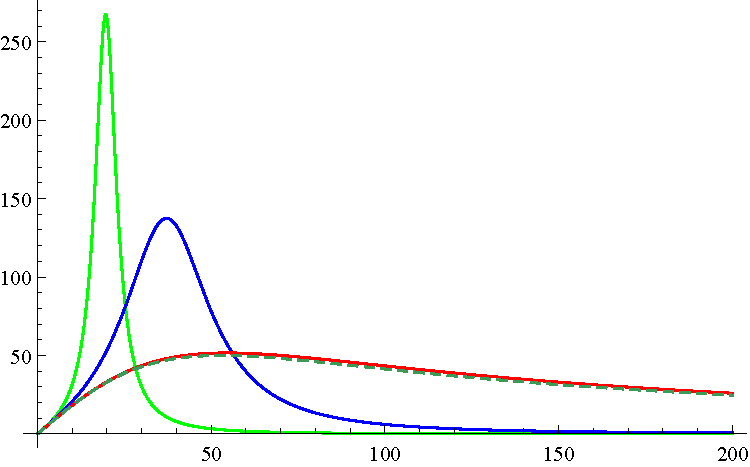
\includegraphics[width=0.5\textwidth]{Images/SDs/SpectralDensities.pdf}
	\caption{Comparison of underdamped (solid lines) and overdamped (dashed line) spectral densities. Parameters are $\omega_c=53cm^{-1}$, $\alpha=100cm^{-1}$ and $\Gamma=\omega_0^2\omega_c^{-1}$.}
\end{figure}
\subsection{The reaction coordinate master equation}
Defining $A= (a + a^{\dagger})$, we get the master equation
\begin{align}
	\begin{split}
		\label{eq:ReactionMasterExpansion4}
		\pdv{\rho(t)}{t} &= -i\left[H_0, \rho(t)\right]\\
		&-\int_{0}^{\infty}\int_{0}^{\infty}d\omega d\tau 
		\left[A,\left[\tilde{A}(-\tau),\rho(t) \right]\right] J_{RC}(\omega) \coth(\frac{\beta \omega}{2})\cos(\omega \tau)\\ 
		-& i\int_{0}^{\infty}\int_{0}^{\infty}d\omega d\tau\left[A ,\biggr\lbrace\left[\tilde{A}(-\tau),H_0\right],\rho(t) \biggr\rbrace \right] J_{RC}(\omega) \frac{\cos(\omega \tau)}{\omega}.
	\end{split}
\end{align}
At this point we can include the integrals over $\tau$ and $\omega$ in the definitions of two new operators
\begin{align}
	\label{eq:NewRCOperators}
	\chi &\equiv \int_{0}^{\infty}\int_{0}^{\infty}d\omega d\tau  J_{RC}(\omega) \coth(\frac{\beta \omega}{2})\cos(\omega \tau) \tilde{A}(-\tau)\\
	\Xi &\equiv \int_{0}^{\infty}\int_{0}^{\infty}d\omega d\tau  J_{RC}(\omega) \frac{\cos(\omega\tau)}{\omega} \left[H_0, \tilde{A}(-\tau)\right]
\end{align}
We then write the system operators in the basis of RC-TLS eigenstates $\ket{\phi_n}$ which gives
\begin{equation}
A = \sum_{ij}\bra{\phi_i}A\ket{\phi_j} \dyad{\phi_i}{\phi_j}
\end{equation}
where $H_0\ket{\phi_n} = \phi_n\ket{\phi_n}$. Transforming to the interaction picture with respect to $H_0$, the system operators become
\begin{equation}
\tilde{A}(t) = \sum_{ij}\bra{\phi_i}A\ket{\phi_j} e^{i(\phi_i-\phi_j)t}\dyad{\phi_i}{\phi_j}.
\end{equation}

Substituting this into (\ref{eq:NewRCOperators}) and integrating using 
\begin{equation}
	\label{eq:Sokhotski}
	\int_{0}^{\infty}f(\omega)d\omega\int_{0}^{\infty}d\tau e^{\pm i(\omega-\eta)\tau} = \pi\int_{0}^{\infty}f(\omega)\delta(\omega-\eta)d\omega \pm i \mathcal{P}\left[\int_{0}^{\infty}\frac{f(\omega)}{\omega-\eta}d\omega\right],
\end{equation}
yields
\begin{align}
	\label{eq:NewRCOperatorsDiscrete}
	\chi &\approx \sum_{ij}J_{RC}(\xi_{ij}) \coth(\frac{\beta \xi_{ij}}{2})\bra{\phi_i}A\ket{\phi_j}\dyad{\phi_i}{\phi_j}\\
	\Xi &\approx \sum_{ij}J_{RC}(\xi_{ij}) \bra{\phi_i}A\ket{\phi_j}\dyad{\phi_i}{\phi_j}
\end{align}
where $\xi_{ij} = (\phi_i-\phi_j)$ and the imaginary Lamb-shift terms have been neglected, justified in \cite{OriginalRCJakeAhsan} by benchmarking. These operators can be calculated by numerically diagonalising the TLS-RC system Hamiltonian $H_0$. This allows us to write the Reaction Coordinate master equation as
\begin{equation}
\pdv{\rho(t)}{t} = -i\left[H_0, \rho(t)\right] - \left[A, \left[\chi, \rho(t)\right]\right] + \left[A, \big\lbrace\Xi, \rho(t)\big\rbrace\right].
\end{equation}
\begin{itemize}
	\item One picture showing the plot of eigenenergies with small $\omega_0$ and one with very large $\omega_0$. Does an underdamped SD give more localised vibration-like manifolds?
	\item Picture showing the dynamics of the coherences in underdamped and overdamped case. Check dynamics of reaction coordinates too.
	\item What do these manifolds mean in the context of the reaction coordinate mapping? How can the decay between vibrational levels be interpreted? Does it accurately represent the physics? (i.e. are the of the low-frequency delocalised phonons strongly coupled to the system in biomolecular systems?)
\end{itemize}

\subsection{Drude-Lorentz Spectral Density (Delocalised phonons)}


\subsection{Underdamped Lorentzian Spectral Density (Localised vibrations)}

\section{Vibronic dissipation due to an electromagnetic bath}
\begin{itemize}
	\item I don't know whether to order the different theories from most severe approximation (electronic) to least severe (non-RWA non-Secular), or the way round that I've done it.
\end{itemize}
\begin{equation}
H = \epsilon \dyad{X} + \sum_{k}h_k(a^{\dagger}+a)(c^{\dagger}_k+c_k) + \sum_{k}\omega_k c^{\dagger}_k c_k + \sum_{j}\sigma_x(g^*_jb^{\dagger}_j+g_jb_j) + \sum_{j}\omega_j b^{\dagger}_jb_j,
\end{equation}
We being by looking at the model of a single electronic molecular transition coupled to a broadened vibrational mode, where the electronic transition is coupled to the surrounding electromagnetic environment. The total Hamiltonian is of the form
\begin{equation}
H = \epsilon \dyad{X} + \eta a^{\dagger}a + \lambda\sigma_z(a^{\dagger}+a) + \sum_{k}h_k(a^{\dagger}+a)(c^{\dagger}_k+c_k) + \sum_{k}\omega_k c^{\dagger}_k c_k + \sum_{j}\sigma_x(g^*_jb^{\dagger}_j+g_jb_j) + \sum_{j}\omega_j b^{\dagger}_jb_j,
\end{equation}
where the first five terms constitute the electronic and vibrational degrees of freedom and the couplings between them and the final two terms are the interaction of the electronic part and the optical bath. If we consider the electronic transition and vibrational mode to be the system of interest we can deal with the system-bath interactions in an open-quantum systems framework,
\begin{equation}
H = H_S + H_I^{Vib} + H_B^{Vib} + H_I^{EM}+ H_B^{EM}
\end{equation}
where 
\begin{equation}
H_S = \epsilon \dyad{X} + \eta a^{\dagger}a + v\sigma_x(a^{\dagger}+a)
\end{equation}
and the rest is self-explanatory for now.
\begin{equation}
J (\omega)= \sum_{j}\abs{g_{\textbf{j}}}^2 \delta (\omega-\omega_j).
\end{equation}
Now we derive four different master equations to describe the dissipative dynamics under different levels of secular approximation. Firstly, we do not make a rotating wave approximation on the system-bath Hamiltonian. This is 
\subsection{Non-Rotating Wave Approximation}
\label{ssec:nrwa}
Here we derive a Born-Markov master equation (Redfield equation) for the light-matter coupling without imposing the rotating wave approximation. The idea is that since the coupled system-vibrational Hamiltonian has potentially degenerate eigenfrequencies spanning many orders of magnitude there may exist some combination of transitions which become non-negligibly coupled by the shared optical field which are \textit{counter-rotating} but slowly. The Hamiltonian for the dissipative vibronic system is $H = H_S + H_B^{Vib} + H_I^{Vib} + H_B^{EM} + H_I^{EM}$
\begin{align}
\label{eq:H_nrwa}
	\begin{split}
		H_S &= \epsilon \sigma^{\dagger}\sigma\otimes I_{RC} + \eta\sigma^{\dagger}\sigma(c + c^{\dagger}) + \Omega ( I_{TLS}\otimes c^{\dagger}c) \\
		H_B^{EM} &= \sum_{j}\omega_j b^{\dagger}_j b_j \quad \quad H_I^{EM} = \sum_{j}(\sigma+\sigma^{\dagger})(g_j^*b^{\dagger}_j+ g_j b_j).
	\end{split}
\end{align}
From this we derive a master equation in the Born-Markov approximation for an weakly-coupled system-bath interaction $H_I(t)$ of arbitrary form
\begin{equation}
\pdv{\rho(t)}{t} = -i[H_S, \rho_S(t)] -\int_{0}^{\infty}d\tau\tr\left(\left[H_I, H_I(-\tau)\rho(t)\right] - \left[H_I, \rho(t)H_I(-\tau)\right]\right)
\end{equation}
where we are integrating over all time-differences $\tau$ by assuming a separation of time-scales between the system dynamics and the bath correlations, we have also assumed that the full density operator is separable $\tilde{\rho}(t) = \tilde{\rho_S}(t)\otimes\tilde{\rho_B}(t)$ for all times $t$. Since we are concerned with the interaction between the system of interest and the electromagnetic field, we transform $H_I^{EM}$ to the interaction picture with respect to the $H_S + H_B$ which accounts for the full vibronic eigenstructure. Here we take advantage of the fact that the interaction Hamiltonian is of the form $H_I^{EM}=AB$ where $A \equiv \sigma + \sigma^{\dagger}$ and $B\equiv \sum_{j}(g_j^*b^{\dagger}_j+ g_j b_j)$ and the fact that $H_B$ and $H_S$ commute.
Eventually we get
\begin{equation}
\label{nRWA_master}
\pdv{\rho(t)}{t} = -i[H_S, \rho_S(t)] - \left[\sigma_x, Z\rho_S(t)\right] - \left[\rho_S(t) Z^{\dagger}, \sigma_x\right]
\end{equation}
where
\begin{equation}
Z = \int_{0}^{\infty}d\tau C(\tau)A(-\tau)
\end{equation}
and
\begin{equation}
C(\tau) = \int_{0}^{\infty}d\omega J(\omega)\left(\coth(\frac{\beta \omega}{2}) \cos\omega\tau - i\sin\omega\tau\right).
\end{equation}
We can calculate the operator $Z$ numerically by expressing the system operator in terms of eigenstates of $H_S$ such that $H_S\ket{\varphi_m}=\varphi_m\ket{\varphi_m}$ so we have
\begin{equation}
\label{eq:Adecomposition}
A(t) = \sum_{m,n} A_{m,n} e^{i\xi_{mn}t}\dyad{\varphi_m}{\varphi_n}.
\end{equation}
In reality, this means we will have to truncate the Hilbert space of the RC. Bringing this all together yields
\begin{equation}
Z = \sum_{m,n} A_{m,n} \int_{0}^{\infty}d\tau \int_{0}^{\infty}d\omega J(\omega)\left(\coth(\frac{\beta \omega}{2}) \cos\omega\tau - i\sin\omega\tau\right)e^{-i\xi_{mn}t}\dyad{\varphi_m}{\varphi_n}
\end{equation}
which can be rewritten as
\begin{equation}
Z = \sum_{m,n} A_{m,n} \Gamma(\xi_{mn}) \dyad{\varphi_m}{\varphi_n}
\end{equation}
where the temperature-dependent rates are defined
\begin{equation}
\Gamma(\xi_{mn}) = \int_{0}^{\infty}d\tau \int_{0}^{\infty}d\omega \left(f_1(\omega)e^{i(\omega-\xi_{mn})\tau} + f_2(\omega)e^{-i(\omega+\xi_{mn})\tau}\right)
\end{equation}
along with the functions
\begin{equation}
f_1(\omega) = \frac{1}{2}J(\omega)(\coth(\beta \omega/2)-1) \quad \textnormal{and} \quad f_2(\omega)= \frac{1}{2}J(\omega)(\coth(\beta \omega/2)+1).
\end{equation}
The rates can be evaluated using \ref{eq:Sokhotski}
\begin{equation}
\Gamma(\xi_{mn}) =
\begin{cases}
\pi f_1(\xi_{mn}) + i\mathcal{P}\left[\int_{0}^{\infty}\left(\frac{f_1(\omega)}{\omega-\xi_{mn}} - \frac{f_2(\omega)}{\omega+\xi_{mn}}\right)d\omega\right] & \text{if } \xi_{mn}>0,\\ 
\frac{\pi}{2}\lim\limits_{x\to 0}\left(J(x)\coth(\frac{\beta x}{2})\right) - i\mathcal{P}\left[\int_{0}^{\infty}\frac{J(\omega)}{\omega}d\omega\right] & \text{if } \xi_{mn}=0,\\ 
\pi f_2(\abs{\xi_{mn}}) + i\mathcal{P}\left[\int_{0}^{\infty}\left(\frac{f_1(\omega)}{\omega+\abs{\xi_{mn}}} - \frac{f_2(\omega)}{\omega-\abs{\xi_{mn}}}\right)d\omega\right]  & \text{if } \xi_{mn}<0.
\end{cases}
\end{equation}
\begin{itemize}
	\item Limiting case: check for a TLS (no vibronic levels) what the master equation terms reduce to. Is there a way to make these terms have negligible effect, as in Ahsan's notes where $\alpha\ll \epsilon$. What would this mean for the vibronic system and which parameter regimes might satisfy this?
	\item What happens if you make the secular approximation? This is not possible for this master equation because I never looked at things in the interaction picture. Would we be interested in studying this?
\end{itemize}
\subsection{Vibronic non-secular theory}
\label{ssec:nsec}
Starting from \ref{eq:H_nrwa} we make a Rotating-Wave-Approximation (RWA) by discarding the counter rotating terms in the $H^{EM}_I$, yielding
\begin{align}
	\begin{split}
		H_S &= \epsilon \sigma^{\dagger}\sigma\otimes I_{RC} + \eta\sigma^{\dagger}\sigma(c + c^{\dagger}) + \Omega ( I_{TLS}\otimes c^{\dagger}c) \\
		H_B^{EM} &= \sum_{j}\omega_j b^{\dagger}_j b_j \quad \quad H_I^{EM} = \sum_{j}g_j\sigma b^{\dagger}_j+ g_j^*\sigma^{\dagger} b_j 
	\end{split}
\end{align}
We transform the interaction Hamiltonian to the interaction picture by $H_I(t) = e^{i(H_S+H_B) t}H_I e^{-i (H_S+H_B)t}$ which gives the form of coupling
\begin{equation}
\label{eq:IDecomposition}
H_I(t) = A(t) B^{\dagger}(t) + A^{\dagger}(t) B(t)  
\end{equation}
where $A(t) = e^{iH_S t}Ae^{-i H_S t}$, $A \equiv\sigma_\otimes I_{RC}$ and $B(t)= \sum_{j}g_ja_je^{-i\omega_j t}$. Since $H_S$ is a composite of two interacting subsystems, it is not straightforward to perform the matrix exponentiation and becomes useful to write down the system operator $A$ in terms of the eigenstates of $H_S$,
\begin{equation}
A \equiv \sigma\otimes I_{RC} = \sum_{m,n} \bra{\varphi_m}\sigma\otimes I_{RC}\ket{\varphi_n}\dyad{\varphi_m}{\varphi_n}
\end{equation}
such that $H_S\ket{\varphi_m}=\varphi_m\ket{\varphi_m}$. So we have the system operator as a superposition of various oscillatory components
\begin{equation}
\label{eq:Adecomposition}
A(t) = \sum_{m,n} A_{m,n} e^{i\xi_{mn}t}\dyad{\varphi_m}{\varphi_n}
\end{equation}
where $\xi_{mn} = \varphi_m - \varphi_n$ and $A_{m,n} = \bra{\varphi_m}A\ket{\varphi_n}$. When the interaction Hamiltonian can be written in this form, the second-order Born-Markov master equation can be expressed
\begin{align}
	\begin{split}
		\label{eq:BornMarkov}
		\pdv{\tilde{\rho}(t)}{t} = - \int_{0}^{\infty}& d\tau  \left[A(t), A^{\dagger}(t-\tau)\tilde{\rho}(t)\right] \expval{B^{\dagger}(\tau)B} + \left[A^{\dagger}(t),A(t-\tau)\tilde{\rho}(t)\right] \expval{B(\tau)B^{\dagger}} + h.c.,
	\end{split}
\end{align}
then substituting \ref{eq:Adecomposition} into this expression we get
\begin{align}
	\begin{split}
		\pdv{\tilde{\rho}(t)}{t} = - \sum_{l,m,p,q}\int_{0}^{\infty}& d\tau e^{-i(\xi_{lm}-\xi_{pq})t} e^{-i\xi_{pq}\tau} A_{l,m}A_{p,q}^{*}\big[\dyad{\varphi_l}{\varphi_m}, \dyad{\varphi_q}{\varphi_p}\tilde{\rho}(t)\big] \expval{B^{\dagger}(\tau)B} \\
		&+ e^{i(\xi_{lm}-\xi_{pq})t} e^{i\xi_{pq}\tau} A_{l,m}^{*}A_{p,q}\big[\dyad{\varphi_m}{\varphi_l}, \dyad{\varphi_p}{\varphi_q}\tilde{\rho}(t)\big] \expval{B(\tau)B^{\dagger}} + h.c.,
	\end{split}
\end{align}
where $A_{l,m}^*=\bra{\varphi_m}A^{\dagger}\ket{\varphi_l}$. The correlation functions can be written as
\begin{align}
	\begin{split}
		\expval{B^{\dagger}(\tau)B} = \tr\left(\sum_{k,k^{\prime}}e^{i\omega_k \tau}g_k^*g_{k^{\prime}} b_k^{\dagger}b_{k^{\prime}}\rho_E\right)\\
		\expval{B(\tau)B^{\dagger}}=\tr\left(\sum_{k,k^{\prime}}e^{-i\omega_k \tau}g_k^*g_{k^{\prime}} b_{k^{\prime}}b_k^{\dagger}\rho_E\right)
	\end{split}
\end{align}
which, after moving to the continuum limit in the number of environmental modes become;
\begin{align}
	\begin{split}
		\expval{B^{\dagger}(\tau)B} = \int_0^{\infty}d\omega e^{i\omega \tau}J(\omega)N(\omega)\\
		\expval{B(\tau)B^{\dagger}}=\int_0^{\infty}d\omega e^{-i\omega \tau}J(\omega)(N(\omega)+1)
	\end{split}
\end{align}
where $J(\omega)$ is the spectral density and $N(\omega)$ is the boson occupation number. From the delta function in \ref{eq:Sokhotski} real part of the integrals over time and frequency become decay rates evaluated at the differences in eigenfrequencies,
\begin{equation}
\gamma(\omega)=\pi J(\omega),
\end{equation}
the imaginary parts are the principal values of the integral which we denote $\Lambda_1$ and $\Lambda_2$. I'll leave these completely for now, but it's only important to know that the integrand of $\Lambda_2$ is $ \propto N(\omega)$ so disappear at zero temperature.
Moving back to the Schrodinger picture gives

\begin{align}
	\label{eq:VibronicNonSecular1}
	\begin{split}
		\pdv{\rho(t)}{t} = -i[H_S, \rho_S(t)] &- \sum_{l,m,p,q}  (N(\xi_{pq})\gamma(\xi_{pq})+i\Lambda_2(\xi_{pq})) A_{l,m}A_{p,q}^{*}\big[\dyad{\varphi_l}{\varphi_m}, \dyad{\varphi_q}{\varphi_p}\tilde{\rho}(t)\big] \\
		&+ (\gamma(\xi_{pq})(N(\xi_{pq})+1)-i(\Lambda_1(\xi_{pq})+\Lambda_2(\xi_{pq})))  A_{l,m}^{*}A_{p,q}\big[\dyad{\varphi_m}{\varphi_l}, \dyad{\varphi_p}{\varphi_q}\tilde{\rho}(t)\big]\\ &+ h.c.
	\end{split}
\end{align}
In order to justify the secular approximation in this case, we would have to show that an overdamped spectral density always gives negligible overlap coefficients $A_{l,m}A_{p,q}^{*}$ for nearly resonant transitions $\xi_{lm}\approx \xi_{pq}$.

There is no dipole-moment associated with transitions between vibrational states within the same electronic state manifold, therefore in the uncoupled basis
\begin{align}
	\begin{split}
		\bra{g,n}\sigma\ket{g,m} = \bra{e,n}\sigma\ket{e,m} = 0, \quad \textnormal{for any phonon modes } m,n.
	\end{split}
\end{align}
I predict that for an underdamped spectral density, the small value of $\Omega$ will mean that the two vibrational manifolds will be well separated so there will be no nearly degenerate states on separate manifolds, this should mean that any two transitions with a large overlap coefficient $A_{l,m}A_{p,q}^{*}$ will describe two far from resonance transitions and the secular approximation will be valid.

In reality, numerically calculating each of these terms is going to be expensive, since if the dimension of the Hilbert space of the RC is $D$ there could be $D^4$ terms in the master equation (although many terms will be zero). As we have seen in the RCME, it is possible to hide most of the non-secular information within some newly defined operators so that only a maximum $D^2$ terms need to be calculated. Taking the master equation \ref{eq:BornMarkov} and transforming back to the Schrodinger picture straight away we have
\begin{align}
	\begin{split}
		\label{eq:BornMarkovSchrod}
		\pdv{\rho(t)}{t} = -i[H_S, \rho(t)] - \int_{0}^{\infty}& d\tau  \left[A, A^{\dagger}(-\tau)\rho(t)\right] \expval{B^{\dagger}(\tau)B} + \left[A^{\dagger},A(-\tau)\rho(t)\right] \expval{B(\tau)B^{\dagger}} + h.c.
	\end{split}
\end{align}
We now substitute in \ref{eq:Adecomposition} and bring the integrals into new operators
\begin{align}
	\begin{split}
		\pdv{\rho(t)}{t} = -i[H_S, \rho(t)] - \int_{0}^{\infty}& d\tau  \left[A, \chi_1 \rho(t)\right]  + \left[\rho(t)\chi_2,A\right] + h.c.
	\end{split}
\end{align}
where 
\begin{align}
	\begin{split}
\chi_1 &= \sum_{i j}\int_{0}^{\infty}d\tau\int_{0}^{\infty}d\omega J(\omega)N(\omega)e^{i\omega\tau}A_{i,j}^* e^{i\xi_{mn}t}\dyad{\varphi_m}{\varphi_n} \\
\chi_2 &= \int_{0}^{\infty}d\tau\int_{0}^{\infty}d\omega J(\omega)(1+N(\omega))e^{-i\omega\tau}A_{i,j}^* e^{i\xi_{mn}t}\dyad{\varphi_m}{\varphi_n} 
	\end{split}
\end{align}

\begin{itemize}
	\item State the argument for a secular approximation and then explain why it is not generally valid in this case, with the figure of coefficients versus frequencies - it is the intermediate, nearly resonant region which is important, weight this by the decay rate so that it accounts for the fact that for the secular approximation to be valid the characteristic system frequency $\omega>\gamma$. In my calculations, the spectral density is constant so it doesn't change anything.
	\item In the case of the RC mapping, the effect is caused by a single phonon mode representing the entire bath. The problem is mapped exactly, does this mean these non-secular effects are real? If not, does this mean that dealing with multiple baths are a limitation of the RC model since the dynamics is mapped exactly only with the single bath? Surely if the Hamiltonians commute then it doesn't matter?
	
	
\end{itemize}


Here we derive the master equation which hides the non-secularity in those operators. We don't have as much physical insight when the problem is in this form, but it is far easier to numerically construct the Liouvillian.

\subsection{Vibronic Lindblad theory}
\label{ssec:sec}
Starting from \ref{eq:VibronicNonSecular1} we make the secular approximation anyway. This is to ensure that the map is completely positive and trace preserving, so always gives physical results for the two subsystem density matrices. This is a strong assumption and we are not expecting it to be correct, based on the evidence we have seen in the previous section, we just want to see the effect that the assumption has on the dynamics in various parameter regimes.

\begin{align}
	\label{eq:VibronicSecular1}
	\begin{split}
		\pdv{\rho(t)}{t} = -i[H_S, \rho_S(t)] &- \sum_{p,q}  (N(\xi_{pq})\gamma(\xi_{pq})+i\Lambda_2(\xi_{pq})) A_{p,q}A_{p,q}^{*}\big[\dyad{\varphi_p}{\varphi_q}, \dyad{\varphi_q}{\varphi_p}\tilde{\rho}(t)\big] \\
		&+ (\gamma(\xi_{pq})(N(\xi_{pq})+1)-i(\Lambda_1(\xi_{pq})+\Lambda_2(\xi_{pq})))  A_{p,q}^{*}A_{p,q}\big[\dyad{\varphi_q}{\varphi_p}, \dyad{\varphi_p}{\varphi_q}\tilde{\rho}(t)\big]\\ &+ h.c. \\
	\end{split}
\end{align}
\begin{align}
	\label{eq:VibronicSecular2}
	\begin{split}
		\pdv{\rho(t)}{t} = -i[H_S, \rho_S(t)] &- \sum_{p,q}  (N(\xi_{pq})\gamma(\xi_{pq})+i\Lambda_2(\xi_{pq})) A_{p,q}A_{p,q}^{*}\big(\dyad{\varphi_p}{\varphi_p}\tilde{\rho}(t) - \dyad{\varphi_q}{\varphi_p}\tilde{\rho}(t)\dyad{\varphi_p}{\varphi_q}\big) \\
		&+ (\gamma(\xi_{pq})(N(\xi_{pq})+1)-i(\Lambda_1(\xi_{pq})+\Lambda_2(\xi_{pq})))  A_{p,q}^{*}A_{p,q}\big(\dyad{\varphi_q}{\varphi_q}\tilde{\rho}(t) - \dyad{\varphi_p}{\varphi_q}\tilde{\rho}(t)\dyad{\varphi_q}{\varphi_p}\big)\\ &+ h.c. \\
	\end{split}
\end{align}
Due to the Hermitian conjugate terms, the imaginary parts either cancel out (the final term on each line) or become unitary Hamiltonian-like contributions
\begin{align}
	\label{eq:VibronicSecular2}
	\begin{split}
		\pdv{\rho(t)}{t} = -i[H_S^{\prime}, \rho_S(t)] &- \sum_{p,q}  N(\xi_{pq})\gamma(\xi_{pq}) A_{p,q}A_{p,q}^{*}\big(\{\dyad{\varphi_p}{\varphi_p}, \tilde{\rho}(t)\} - 2\dyad{\varphi_q}{\varphi_p}\tilde{\rho}(t)\dyad{\varphi_p}{\varphi_q}\big) \\
		&+ \gamma(\xi_{pq})(N(\xi_{pq})+1)  A_{p,q}^{*}A_{p,q}\big(\{\dyad{\varphi_q}{\varphi_q}, \tilde{\rho}(t)\} - 2\dyad{\varphi_p}{\varphi_q}\tilde{\rho}(t)\dyad{\varphi_q}{\varphi_p}\big) \\
	\end{split}
\end{align}
here we can see that making the secular approximation has resulted in a summation of many Lindblad operators, with collapse operators formed from the various vibronic eigenstates.

\subsection{Electronic Lindblad theory}
\label{ssec:electronic}
Here we make the most severe approximation, whereby we leave the vibrational degrees of freedom out of the system Hamiltonian altogether. This means that we write the system operators in the master equation in the uncoupled electronic eigenbasis rather than the dressed vibronic eigenbasis. This is akin to introducing the optical and vibrational couplings to the system on the same order, namely that they are both weak and the internal system dynamics can be described accurately by the eigenstructure of the electronic degrees of freedom only. Since we want to calculate the dynamics for the system in

The simplest way to define the dissipation due to the electromagnetic bath is to assume that the interaction energy of electron-vibration coupling is a small parameter so that it's effect can be neglected in the system eigenstructure, therefore we can write down the system operators in the Born-Markov master equation in terms of the electronic system eigenstates only.
\textbf{TODO}
\section{Analysis}
\subsection{Drude-Lorentz Spectral Density (Delocalised phonons)}
Firstly, assuming a flat optical spectrum $J(\omega) = \alpha_{EM}$, high temperature (6000K) and fairly strong coupling (300$cm^{-1}$), see figure \ref{fig:steadyStatevsSplitting}
\begin{itemize}
	\item At large splitting, all three theories converge.
	\item As splitting decreases, the steady state populations of the secular and non-secular theories decrease with respect to the naive. The difference between secular and non-secular increases and the two dip to a local minimum.
	\item Around some small splitting, the secular and non-secular steady states then sharply return to rough agreement with the naive theory (need to make a smoother curve in the small splitting region to properly analyse)
\end{itemize}
When the splitting is small w.r.t. phonon coupling, thermal energy and the width of the phonon distribution, the excitations have more decay pathways due to overlapping vibronic wavefunctions on neighbouring manifolds. This allows the system to reach different lower steady states, with a non-monotonic dependency on splitting. The naive theory does not \emph{see} these vibronic levels, since each manifold is treated like the ground and excited state of the TLS and the dissipation mixes the two.

In single molecular transitions these effects may not be important, since the splittings are often on the order of $8000-20000 cm^{-1}$, so the vibronic manifolds are well defined, with little overlap even at large phonon couplings. In multi-site systems, nearly-resonant neighbouring molecules may interact so that small electronic dipolar transition frequencies are present in the system eigenstructure, this may have a large effect on the steady states.

\begin{figure}[h]
	\centering
	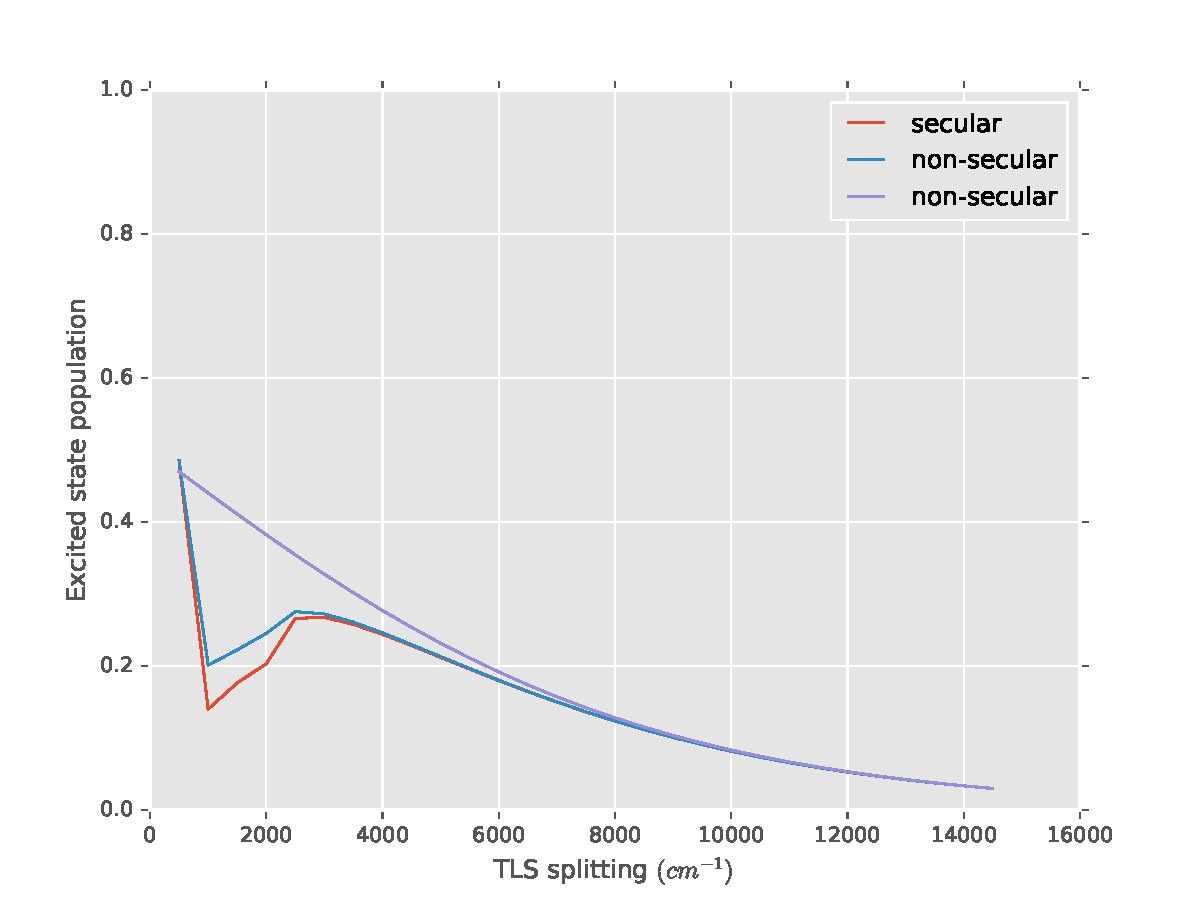
\includegraphics[width=0.8\textwidth]{Images/Checks/Pop_SS_divergence_a300_Tem6000_w0300_eps2000.pdf}
	\caption{Steady-state excited state population as a function of TLS splitting where $\alpha_{ph}=300$, $T_{EM} =6000$, $\omega_0 = 300$}
	\label{fig:steadyStatevsSplitting}
\end{figure}


\subsection{Underdamped Lorentzian Spectral Density (Localised vibrations)}
\begin{itemize}
	\item Large splitting, everything converges.
	\item As splitting decreases, the NS and S start to diverge from the naive. NS and S remain close until very small splitting, at which point the NS appears to return towards agreement with naive.
\end{itemize}

For moderate splitting and an underdamped phonon spectral density, the excited and ground states vibronic manifolds are well separated, see figures \ref{fig:manifold_weakcoupling}-\ref{fig:manifold_strongsmallsplitting}. This means that the dynamics are well approximated by the naive, electronic Lindblad theory of dissipation. However, if the electronic splitting becomes sufficiently small then the two manifolds can overlap and we start to observe the complex behaviour seen in the overdamped case. This happens at a much smaller splitting size since the ladder spacing of the vibronic states is so much smaller.

\begin{itemize}
	\item Is this occurring because the system is so far off resonance with the vibrations? (Reducing the splitting so it is closer to the peak of the spectral density indeed means vibronic theories diverge from the naive.)
\end{itemize}

\begin{figure}[h]
	\centering
	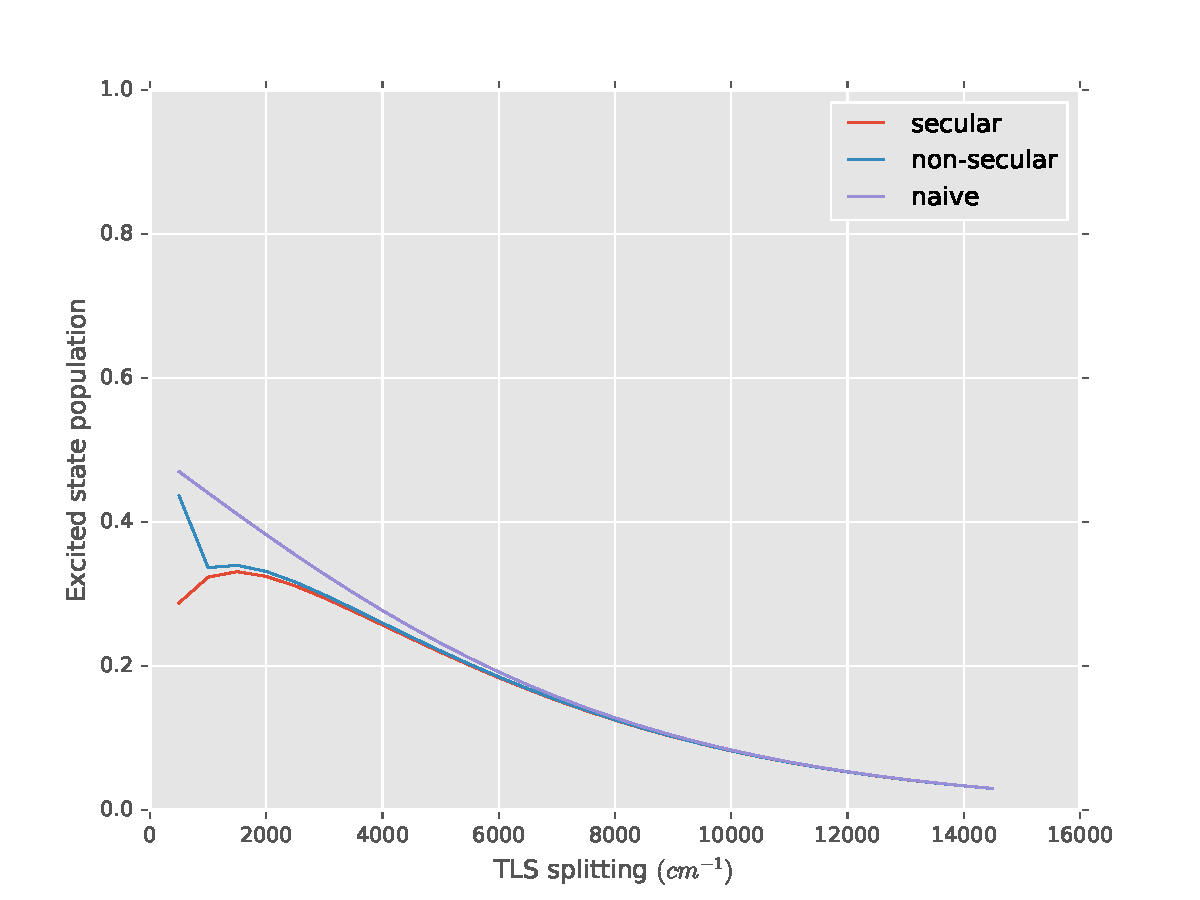
\includegraphics[width=0.8\textwidth]{Images/Checks/RealPop_SS_divergence_a300_Tem6000_w030_eps2000.pdf}
	\caption{Steady-state excited state population as a function of TLS splitting where $\alpha_{ph}=300$, $T_{EM} =6000$, $\omega_0 = 30$, $k_B T_{EM}=4170cm^{-1}$}
	\label{fig:steadyStatevsSplitting}
\end{figure}

\begin{figure}[h]
	\centering
	\begin{minipage}[b]{0.325\textwidth}
		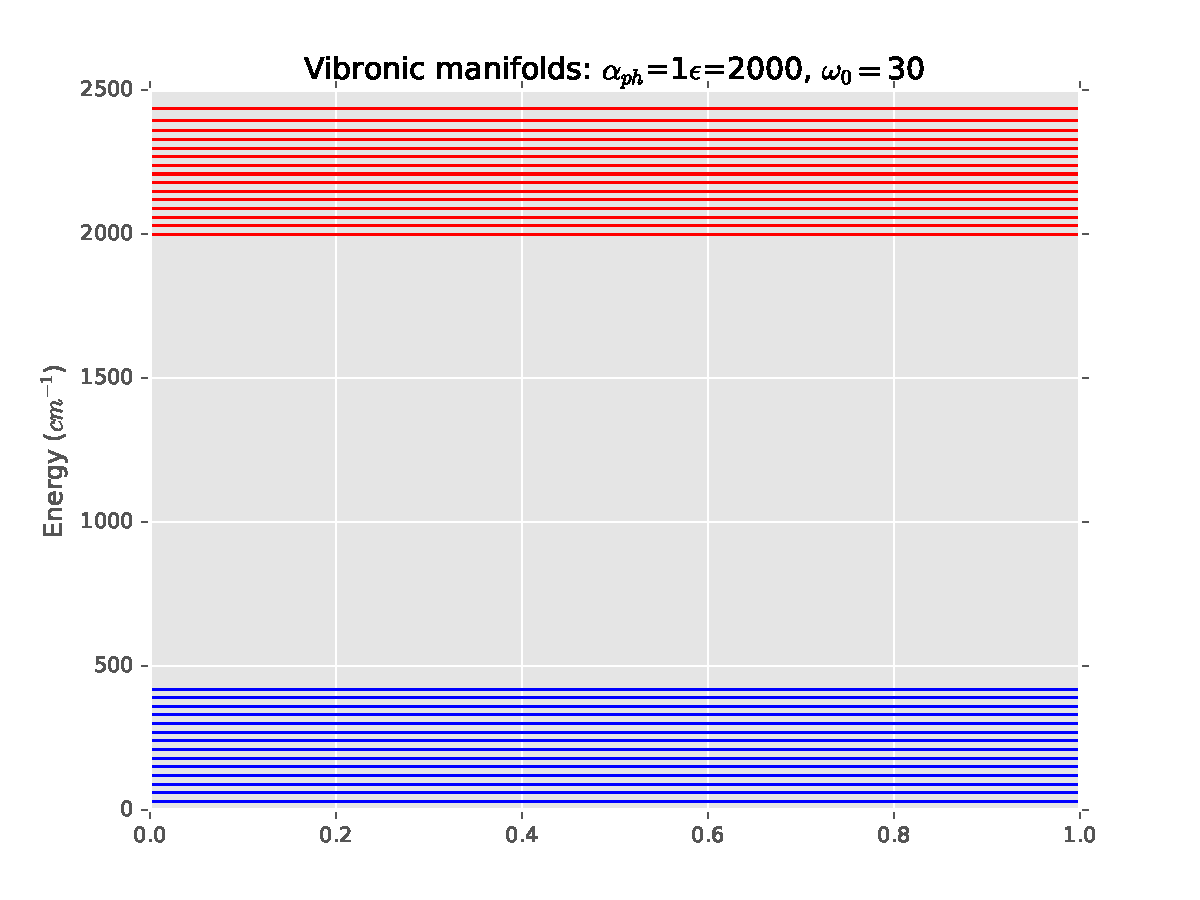
\includegraphics[width=\textwidth]{Images/Spectra/Manifolds_a1_Tph300_Tem6000_w030_eps2000.pdf}
		\caption{}
		\label{fig:manifold_weakcoupling}
	\end{minipage}
	\begin{minipage}[b]{0.325\textwidth}
		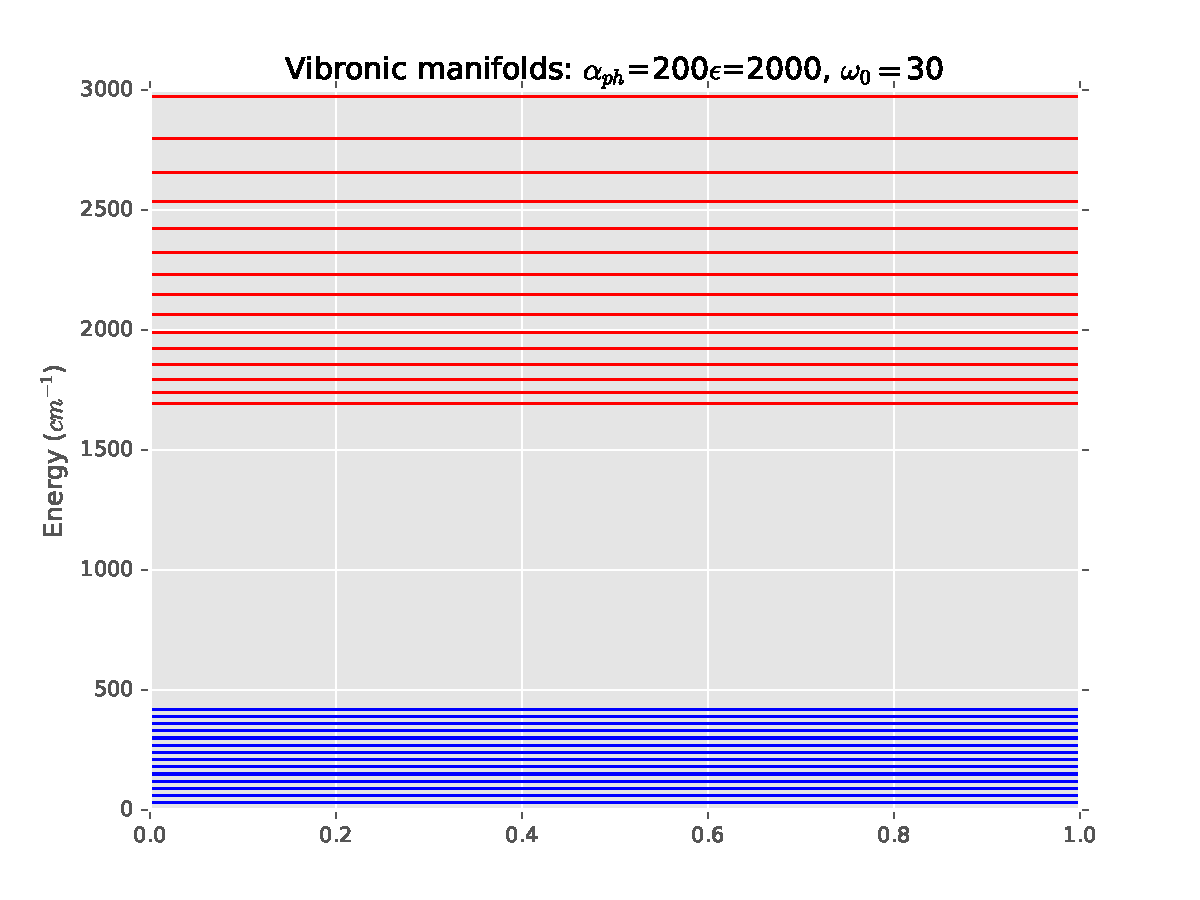
\includegraphics[width=\textwidth]{Images/Spectra/Manifolds_a200_Tph300_Tem6000_w030_eps2000.pdf}
		\caption{}
		\label{fig:manifold_stronglargesplitting}
	\end{minipage}
	\begin{minipage}[b]{0.325\textwidth}
		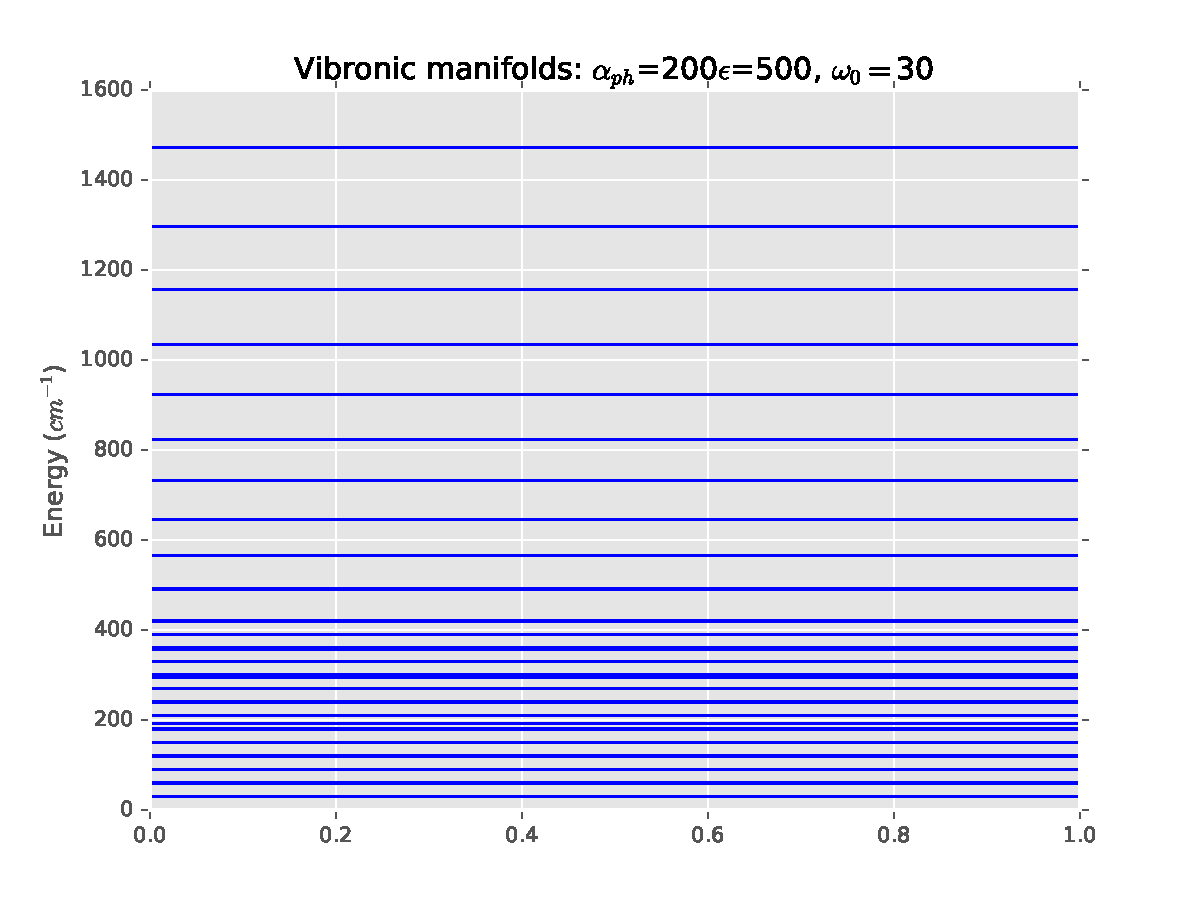
\includegraphics[width=\textwidth]{Images/Spectra/Manifolds_a200_Tph300_Tem6000_w030_eps500.pdf}
		\caption{}
		\label{fig:manifold_strongsmallsplitting}
	\end{minipage}
\caption{The vibronic manifold structure of the TLS with an underdamped Phonon spectral density. It can be seen that strong-coupling as well as small splitting can cause mixing of the vibronic levels.}
\end{figure}
\begin{comment}
\begin{figure}[h]
	\centering
	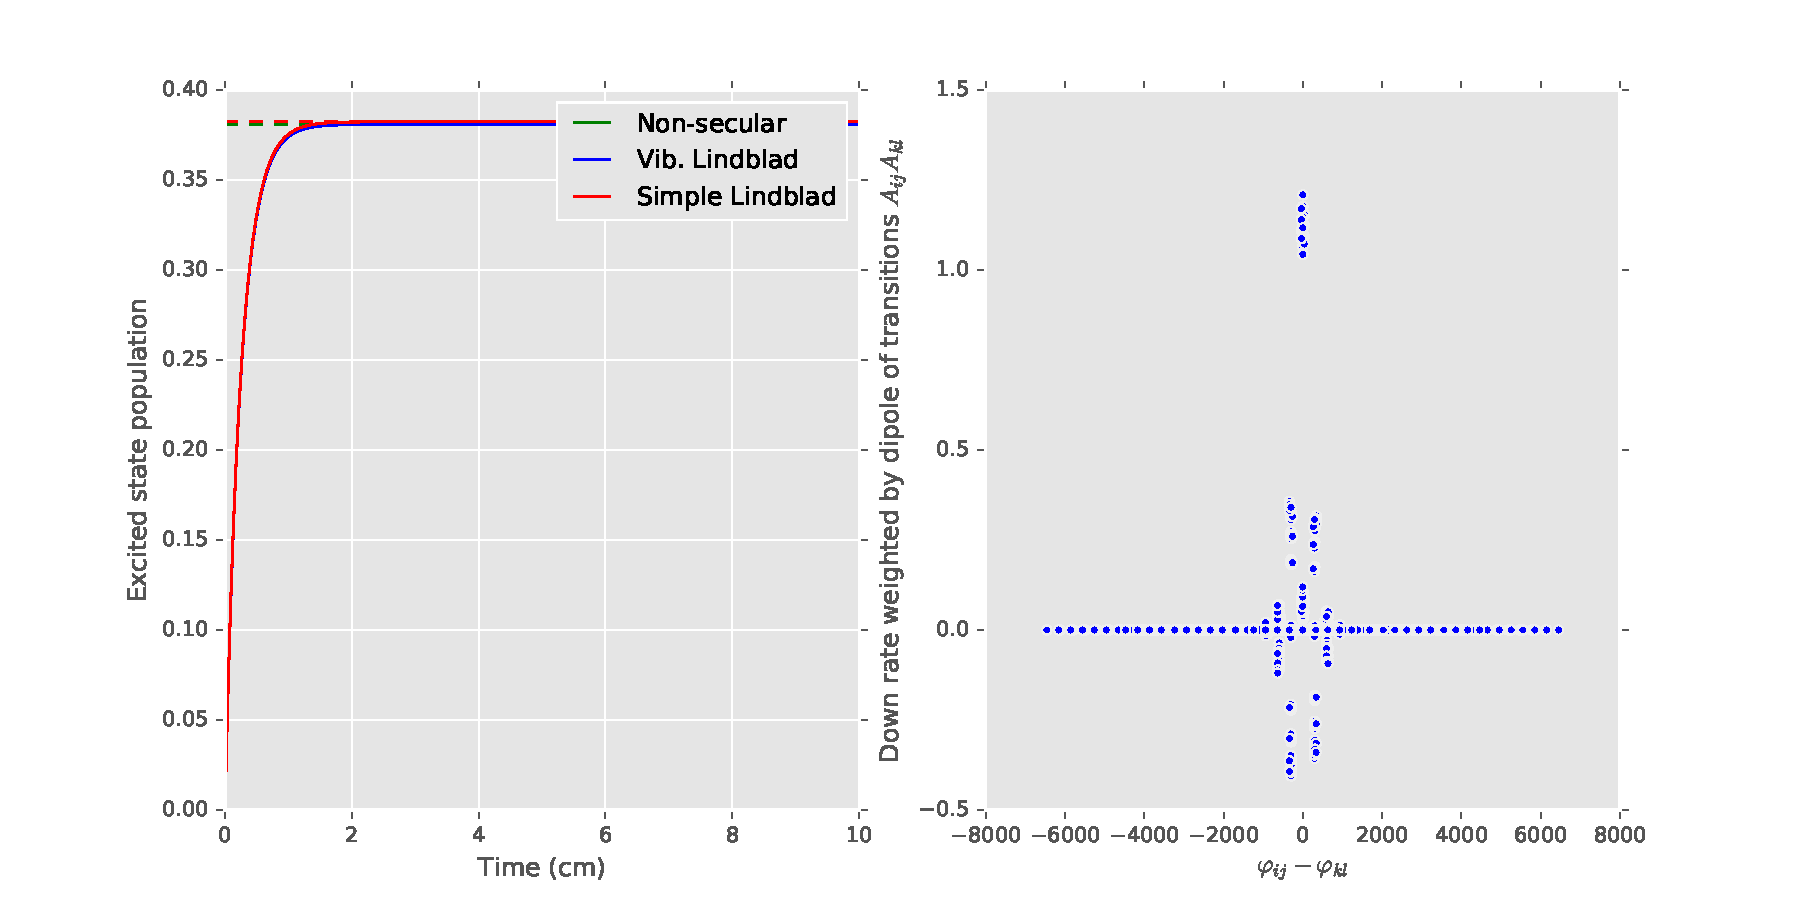
\includegraphics[width=\textwidth]{Images/Dynamics/Pop_a5_N15_Tem6000_w0300_eps2000.pdf}
	\caption{Population where $\alpha_{ph}=5$, $T_{EM} =6000$, $\omega_0 = 300$, $\epsilon=10000$}
	\label{}
\end{figure}
\begin{figure}[h]
	\centering
	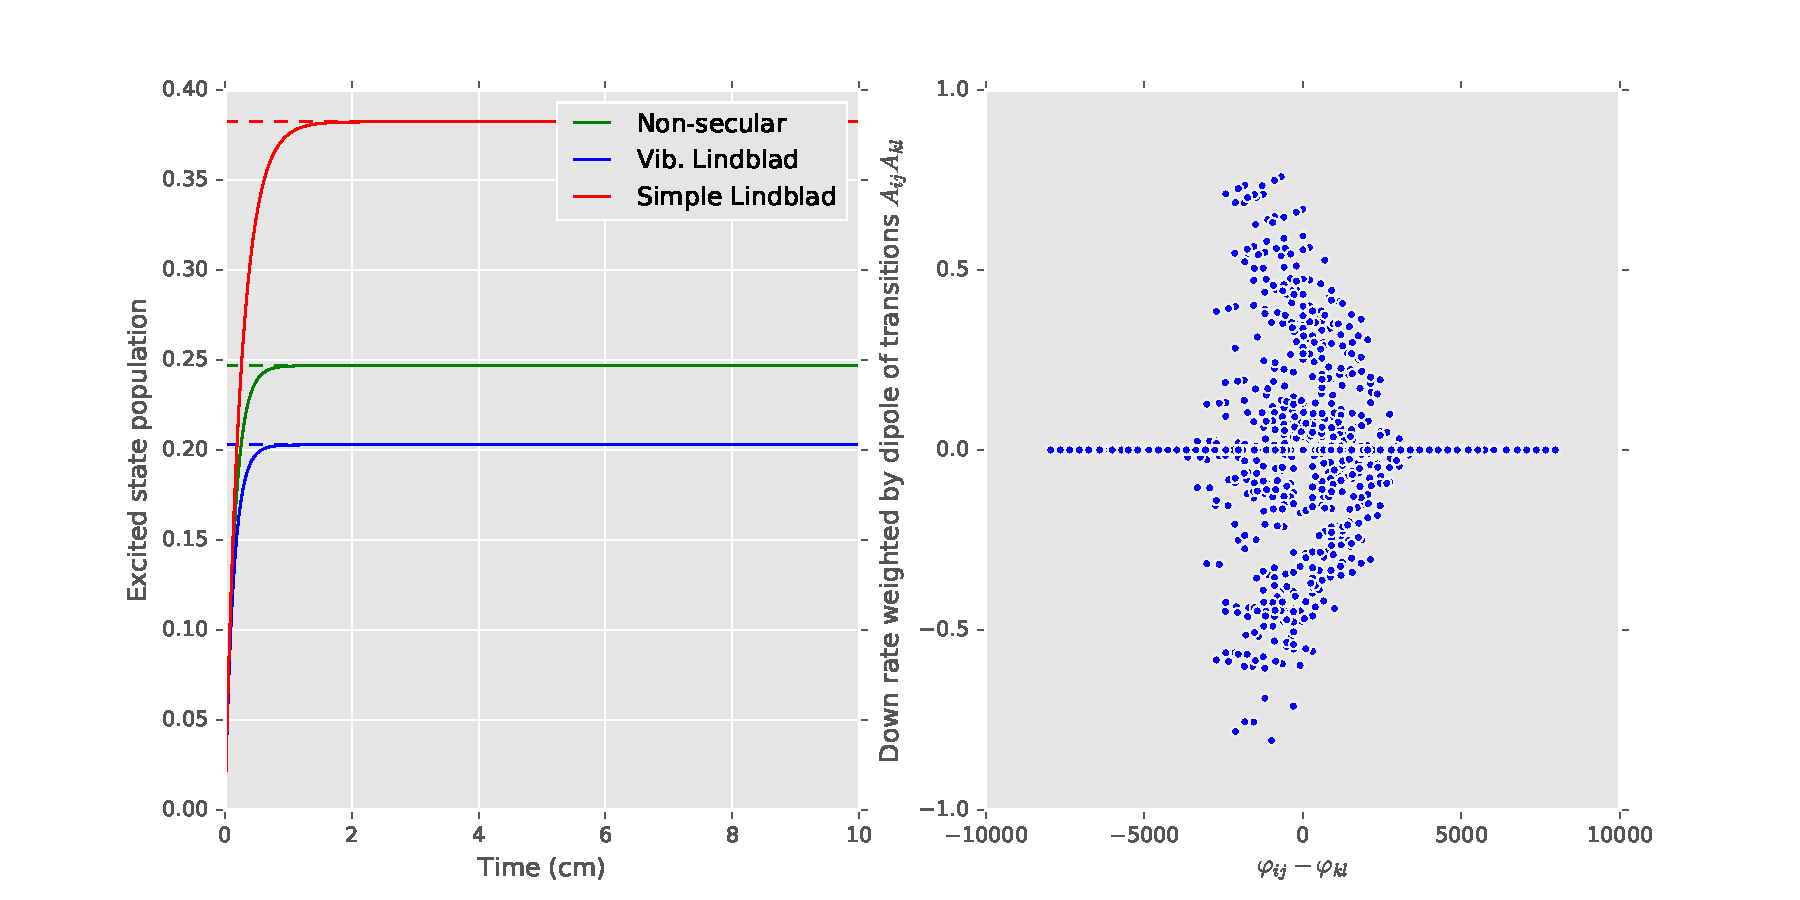
\includegraphics[width=\textwidth]{Images/Dynamics/Pop_a300_N15_Tem6000_w0300_eps2000.pdf}
	\caption{Population where $\alpha_{ph}=300$, $T_{EM} =6000$, $\omega_0 = 300$, $\epsilon=2000$}
	\label{}
\end{figure}
\begin{figure}[h]
	\centering
	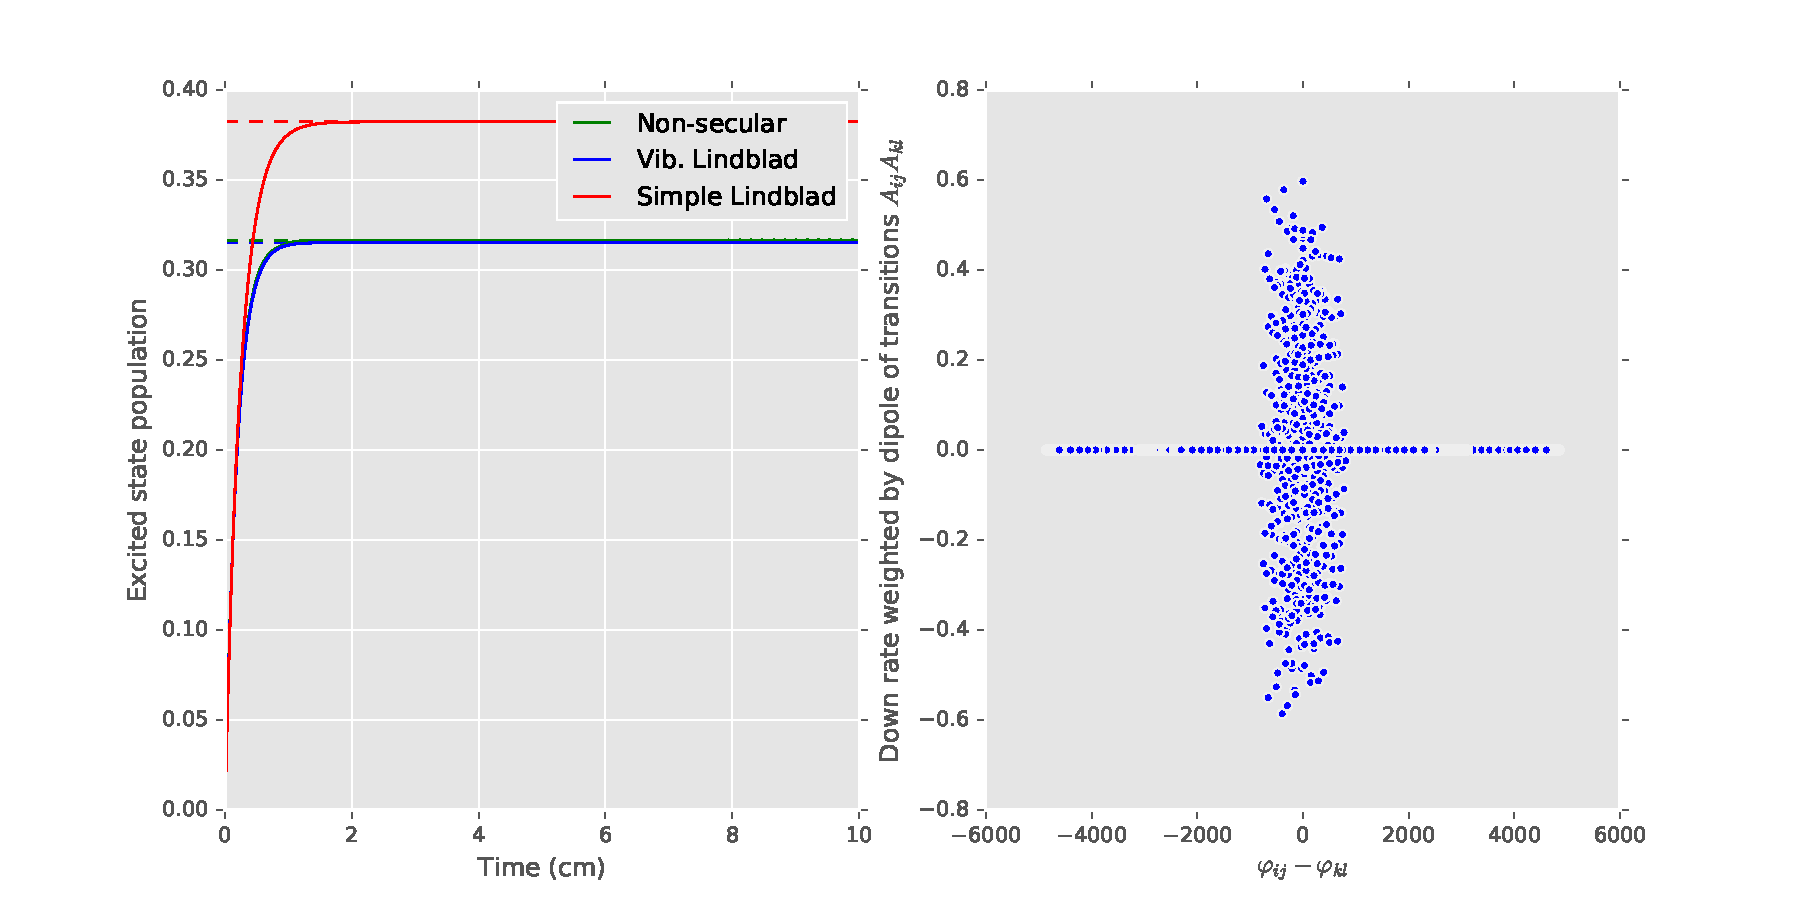
\includegraphics[width=\textwidth]{Images/Dynamics/Pop_a300_N15_Tem6000_w030_eps2000.pdf}
	\caption{Population where $\alpha_{ph}=300$, $T_{EM} =6000$, $\omega_0 = 30$, $\epsilon=2000$}
	\label{}
\end{figure}

\subsection{Validity of RWA}
\begin{itemize}
	\item Comparing \ref{ssec:nrwa} and \ref{ssec:nsec} find regimes where the two different Hamiltonians yield the same dynamics. Within these regimes, do they agree with the secular theories too? Therefore, does secular imply rotating-wave (at least in the dissipators)?
	\item It seems like the underdamped spectral density reduces the temperature dependence of the dynamics. For strong phonon coupling, non-secular is never equivalent to the secular theory.
\end{itemize}
\end{comment}
\section{Future work}

\subsection{Polaron shifts, phonon dynamics and optical spectra}

\begin{itemize}
	\item Does non-secularity alter the dynamics predicted by the Franck-Condon model for $T_{EM}=0$?
	\item As temperature increases, what happens to the equilibrium phonon positions?
	\item Think about polaron shifts. Does this cause the overlaps of excited and ground states to decrease? Does this lead to excessive loss between absorption and emission spectra?
	\item Do the calculations of Fluorescence spectra for electronic and non-secular theories in both the overdamped and underdamped phonon cases. See if the profiles match the theory that they are able to model localised and delocalised vibrations respectively. The electromagnetic bath should be $k_B T\ll \hbar\omega$ to let the vibrational levels decay back to the potential minima of the electronic levels.
\end{itemize}


\bibliographystyle{abbrv}
\bibliography{}
\end{document}
